\documentclass[xcolor={usenames,dvipsnames}]{beamer}
\usepackage[utf8]{inputenc}
\usepackage[english]{babel}

% -- Including some standard packages --
\usepackage{graphicx}
\usepackage{soul}
\usepackage{hyperref}
\usepackage{colortbl}
\usepackage{dsfont}
\usepackage{soul}

% -- Choosing theme --

\usetheme{Boadilla}
\usecolortheme{spruce}
\setbeamercolor{alerted text}{fg=purple} % Making alerted text non-red

% Tikz
\usepackage{tikz,tikz-3dplot,tikz-cd,tkz-tab,tkz-euclide,pgf,pgfplots}
\usetikzlibrary{matrix,positioning,fit,backgrounds,intersections}

% -- Cross signs --
\usepackage{pifont} % http://ctan.org/pkg/pifont
\newcommand{\cmark}{\ding{51}}%
\newcommand{\xmark}{\ding{55}}%
\newcommand{\xopt}{\ding{48}}%

% -- Custom commands --
\DeclareMathOperator*{\argmax}{arg\,max}
\DeclareMathOperator*{\argmin}{arg\,min}

\title[Introduction to ZK]{\textbf{Introduction to Zero-Knowledge Proofs}}
\author{Distributed Lab}
\date{August 22, 2024}
\titlegraphic{
    
\includegraphics[width=\textwidth]{images/banner_wide.png}
}

\expandafter\def\expandafter\insertshorttitle\expandafter{%
  \insertshorttitle\hfill%
  \insertframenumber\,/\,\inserttotalframenumber}

\AtBeginSection[]{
  \begin{frame}
  \vfill
  \centering
  \begin{beamercolorbox}[sep=8pt,center,shadow=true,rounded=true]{title}
    \usebeamerfont{title}\insertsectionhead\par%
  \end{beamercolorbox}
  \vfill
  \end{frame}
}

\begin{document}
	\frame {
		\titlepage
	}
 
	\begin{frame}{Plan}
        \tableofcontents
    \end{frame}

	\section{Introduction}

    \subsection{Classical Proofs}
    \begin{frame}{Classical Proofs}
        \begin{columns}
            % Description
            \begin{column}{0.6\textwidth}
                \begin{itemize}
                    \item First proofs you have probably encountered were \textbf{geometry proofs}. 
                    \item You were given \textbf{axioms} and you can prove certain \textbf{statements} $x$ using them.
                    \item The proof $\pi$ is a sequence of logical steps that lead from axioms to the statement. Essentially, you have a witness $w$ that proves the statement.
                    \item Your teacher is the \textbf{verifier} $\mathcal{V}$ who checks your proof, while you are the \textbf{prover} $\mathcal{P}$.
                    \item This is a \textbf{classical proof} and in a sense, it is a \textbf{non-interactive proof}.
                \end{itemize}
            \end{column}
            % Column 2    
            \begin{column}{0.4\textwidth}
                \begin{figure}
                \centering
                    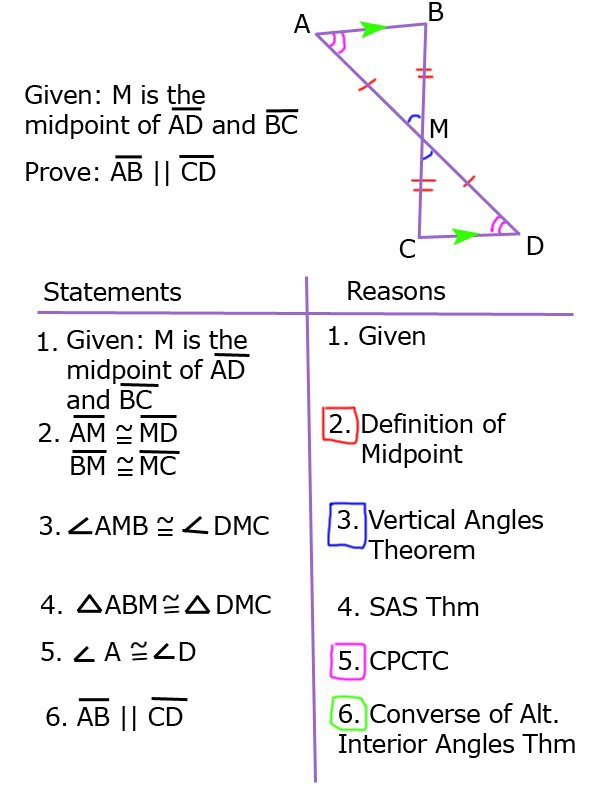
\includegraphics[width=1.0\textwidth]{images/lecture_6/geometry-proof.jpg}
                    \caption{Geometry proof.}
                \end{figure}
            \end{column}
            \end{columns}
    \end{frame}

    \begin{frame}{Motivation}
        \begin{alertblock}{Note}
            However, we cannot use such proofs in the digital world. 
            
            \begin{itemize}
                \item Proofs must be verified by computers. Therefore, we need to develop \textbf{mathematic framework} to be able to program them.
                \item This leads to the question: what is \textbf{statement}? What is \textbf{proof}? What is \textbf{witness}? How to formally define them?
                \item We need to formalize these concepts.
            \end{itemize}
        \end{alertblock}

        \begin{figure}
            \centering
            
\includegraphics[width=0.25\textwidth]{images/lecture_6/thonk.png}
            \caption{Hmm\ldots}
        \end{figure}
    \end{frame}

    \subsection{Goal of the course}
    \begin{frame}{The most basic setting}
        \begin{itemize}
            \item We have a \textbf{prover} $\mathcal{P}$ and a \textbf{verifier} $\mathcal{V}$.
            \item Prover $\mathcal{P}$ wants to prove some statement $x$ to the verifier.
            \item Prover $\mathcal{P}$ has a \textbf{witness} $w$ that contains all necessary information to prove the statement $x$. He sends $\pi$ as a proof.
            \item Verifier $\mathcal{V}$ wants to be convinced that the statement $x$ is true.
        \end{itemize}

        \begin{figure}
            \centering
            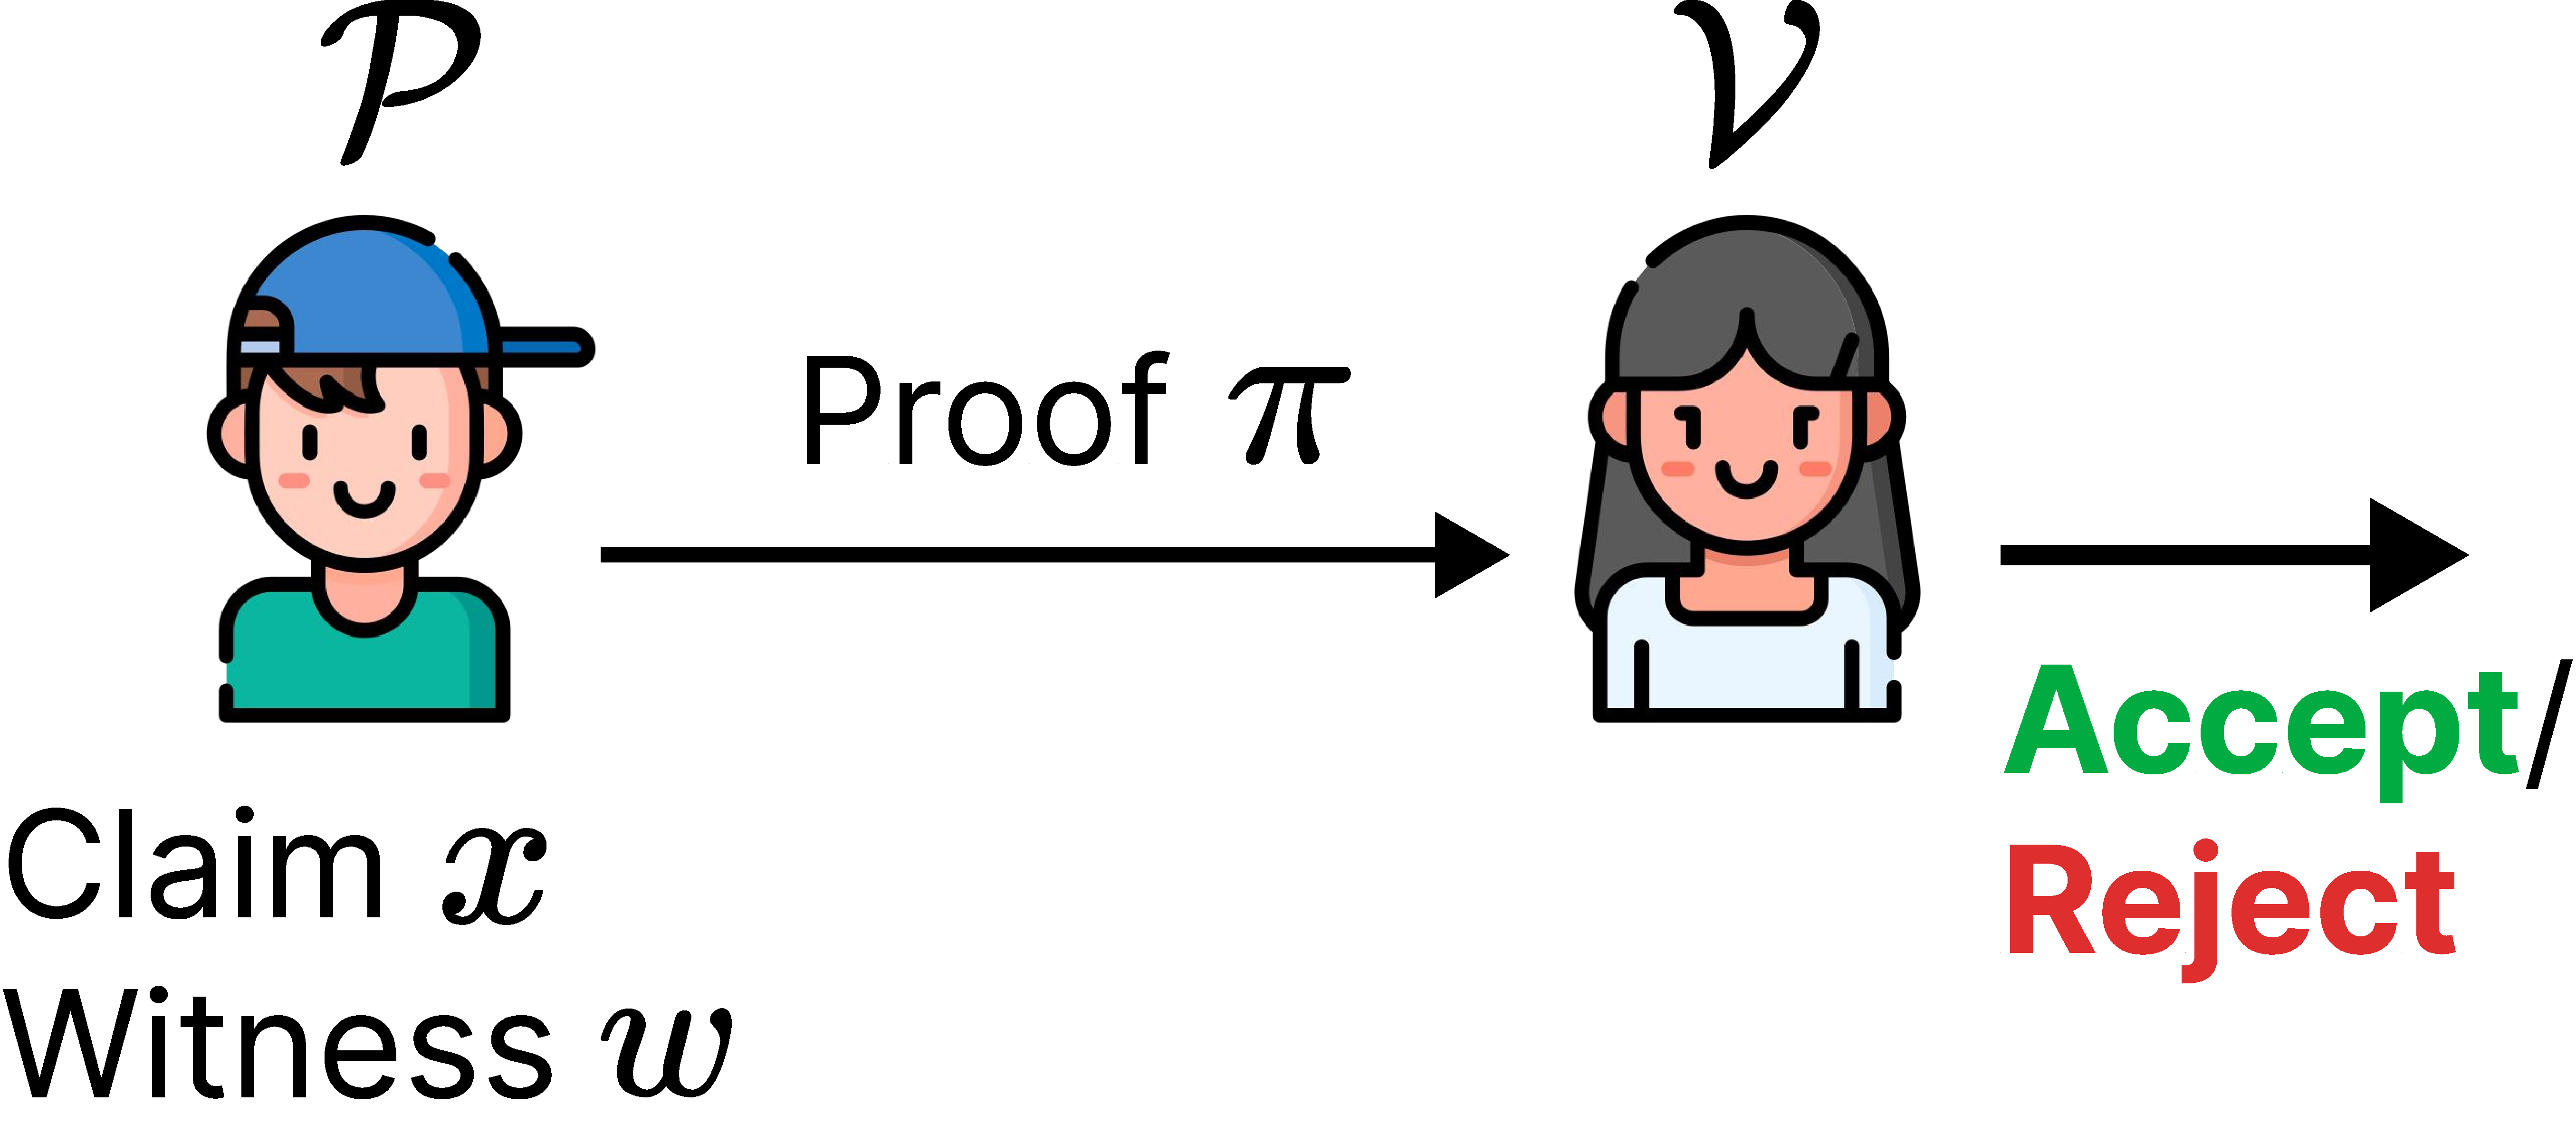
\includegraphics[width=0.7\textwidth]{images/lecture_6/setup.pdf}
            \caption{Typical setup for cryptographic proofs.}
        \end{figure}
    \end{frame}

    \begin{frame}{The Goal of SNARKs, STARKs etc.}
        We will try to solve the following problems:
        \begin{itemize}
            \item \textbf{Completeness:} If $x$ is true, $\pi$ proofs the statement.
            \item \textbf{Soundness:} If $x$ is false, the prover $\mathcal{P}$ should not be able to convince the verifier $\mathcal{V}$ via any $\pi^*$.
            \item \textbf{Zero-knowledge:} $\pi$ does not reveal anything about $w$.
            \item \textbf{Argument of knowledge:} Sometimes, the prover $\mathcal{P}$ should convince the verifier $\mathcal{V}$ that besides $x$ is true, he \textbf{knows} the witness $w$.
            \item \textbf{Succinctness:} The proof should be short, ideally polylogarithmic in the size of the statement ($\pi = \mathsf{polylog}(|x|)$) + fast verification.
            \item \textbf{Arithmetization:} We need to convert the statement $x$ into some algebraic form + make it relatively universal.
        \end{itemize}

        \begin{alertblock}{Note}
            SNARK, STARK, etc. will solve these problems!
        \end{alertblock}
    \end{frame}

    \begin{frame}{Example to demonstrate the goal}
        \begin{example}
            Given a hash function $H: \{0,1\}^* \to \{0,1\}^{\ell}$, $\mathcal{P}$ wants to convince $\mathcal{V}$ that he knows the preimage $x \in \{0,1\}^*$ such that $H(x) = y$.
            \begin{itemize}
                \item \textbf{Zero-knowledge:} The prover $\mathcal{P}$ does not want to reveal \textit{anything} about the pre-image $x$ to the verifier $\mathcal{V}$.
                \item \textbf{Argument of knowledge:} Proving $y$ has a pre-image is useless. $\mathcal{P}$ must show he \textbf{knows} $x \in \{0,1\}^*$ s.t. $H(x)=y$.
                \item \textbf{Succinctness:} If the hash function takes $n$ operations to compute, the proof should be \textbf{much} shorter than $n$ operations. \textbf{State-of-art}: size is $\mathsf{polylog}(n) = O((\log n)^c)$. Verification time is also typically polylogarithmic (or even $O(1)$ in some cases).
            \end{itemize}
        \end{example}

        \begin{block}{Note}
            But first, let us start with the basics.
        \end{block}
    \end{frame}

    \section{Relations. Languages. NP Statements.}

    \subsection{Language of true statements. Examples.}
    \begin{frame}{Language}
        \begin{definition}[Relation]
            Given two sets $\mathcal{X}$ and $\mathcal{Y}$, the \textbf{relation} is $\mathcal{R} \subseteq \mathcal{X} \times \mathcal{Y}$.
            \begin{itemize}
                \item $\mathcal{X}$ is typically a set of \textbf{statements}.
                \item $\mathcal{Y}$ is a set of \textbf{witnesses}.
            \end{itemize}
        \end{definition}

        \begin{definition}[Language of true statements]
            Let $\mathcal{R} \subseteq \mathcal{X} \times \mathcal{Y}$ be a relation. We say that a statement $x \in \mathcal{X}$ is a \textbf{true} statement if $(x,y) \in \mathcal{R}$ for some $y \in \mathcal{Y}$, otherwise the statement is called \textbf{false}. We define by $\mathcal{L}_{\mathcal{R}}$ (the language over relation $\mathcal{R}$) the set of all true statements, that is:
            \begin{equation*}
                \mathcal{L}_{\mathcal{R}} = \{ x \in \mathcal{X}: \exists y \in \mathcal{Y} \; \text{such that} \; (x,y) \in \mathcal{R} \}.
            \end{equation*}
        \end{definition}
    \end{frame}

    \begin{frame}{Language Example \#1: Semiprimes}
        \begin{example}[Product of Two Primes (Semiprimes)]
            \textbf{Claim:} number $n \in \mathbb{N}$ is the product of two prime numbers $w = (p,q) \in \mathbb{N} \times \mathbb{N}$. The \textbf{relation} is given by:
            \begin{equation*}
                \mathcal{R} = \{ (n, p, q) \in \mathbb{N}^3: n = p \cdot q \; \text{where $p,q$ are primes} \}
            \end{equation*}
        
            In this particular case, the \textbf{language of true statements} is defined as 
            \begin{equation*}
                \mathcal{L}_{\mathcal{R}} = \{n \in \mathbb{N}: \exists w=(p,q) \; \text{are primes such that}\; n = p\cdot q\}
            \end{equation*}
            
            \begin{itemize}
                \item \textbf{Valid witness \#1:} $n=15 \in \mathcal{L}_{\mathcal{R}}$. Witness: $w=(3,5)$.
                \item \textbf{Invalid witness:} $n=16 \not\in \mathcal{L}_{\mathcal{R}}$. There is no valid witness.
                \item \textbf{Valid witness \#2:} $n=50252009 \in \mathcal{L}_{\mathcal{R}}$. Witness: $w=(5749,8741)$.
            \end{itemize}
        \end{example}

        \textcolor{purple}{\textbf{Question:}} Is $n=27$ a true statement? What about $n=26$?
    \end{frame}

    \begin{frame}{Language Example \#2: Square Root}
        \begin{block}{Reminder}
            $\mathbb{Z}_N^{\times} = \{x \in \mathbb{Z}_N: \text{gcd}\{x,N\}=1\}$. \textbf{Example:} $\mathbb{Z}_{10}^{\times} = \{1,3,7,9\}$
        \end{block}

        \begin{example}
            \textbf{Claim}: number $x \in \mathbb{Z}_N^{\times}$ is a \textbf{quadratic residue} modulo $N$: $(\exists w \in \mathbb{Z}_N^{\times}): \{x \equiv w^2 \pmod{N}\}$ ($w$ is \textbf{modular square root} of $x$). 
            
            \textbf{Relation}: $\mathcal{R} = \{ (x, w) \in (\mathbb{Z}_N^{\times})^2: x \equiv w^2 \pmod{N} \}$
        
            \textbf{Language:} $\mathcal{L}_{\mathcal{R}} = \{x \in \mathbb{Z}_N^{\times}: \exists w \in \mathbb{Z}_N^{\times} \; \text{such that} \; x \equiv w^2 \pmod{N}\}$. 
            
            \textbf{Examples} for $N=7$: 
            \begin{itemize}
                \item $4 \in \mathcal{L}_{\mathcal{R}}$ since $5^2 \equiv 4 \pmod{7}$. 
                \item $3 \not\in \mathcal{L}_{\mathcal{R}}$ since there is no valid witness for $3$.
            \end{itemize}
        \end{example}

        \textcolor{purple}{\textbf{Question:}} Is $x=1$ a true statement for $N=5$? What about $x=4$?
    \end{frame}

    \begin{frame}{NP Statements: Demonstration}
        Well\ldots We are simply going to send witness $w$ to the verifier $\mathcal{V}$ and he will check if the statement is true (meaning, whether $x \in \mathcal{L}_{\mathcal{R}}$).

        \begin{figure}
            \centering
            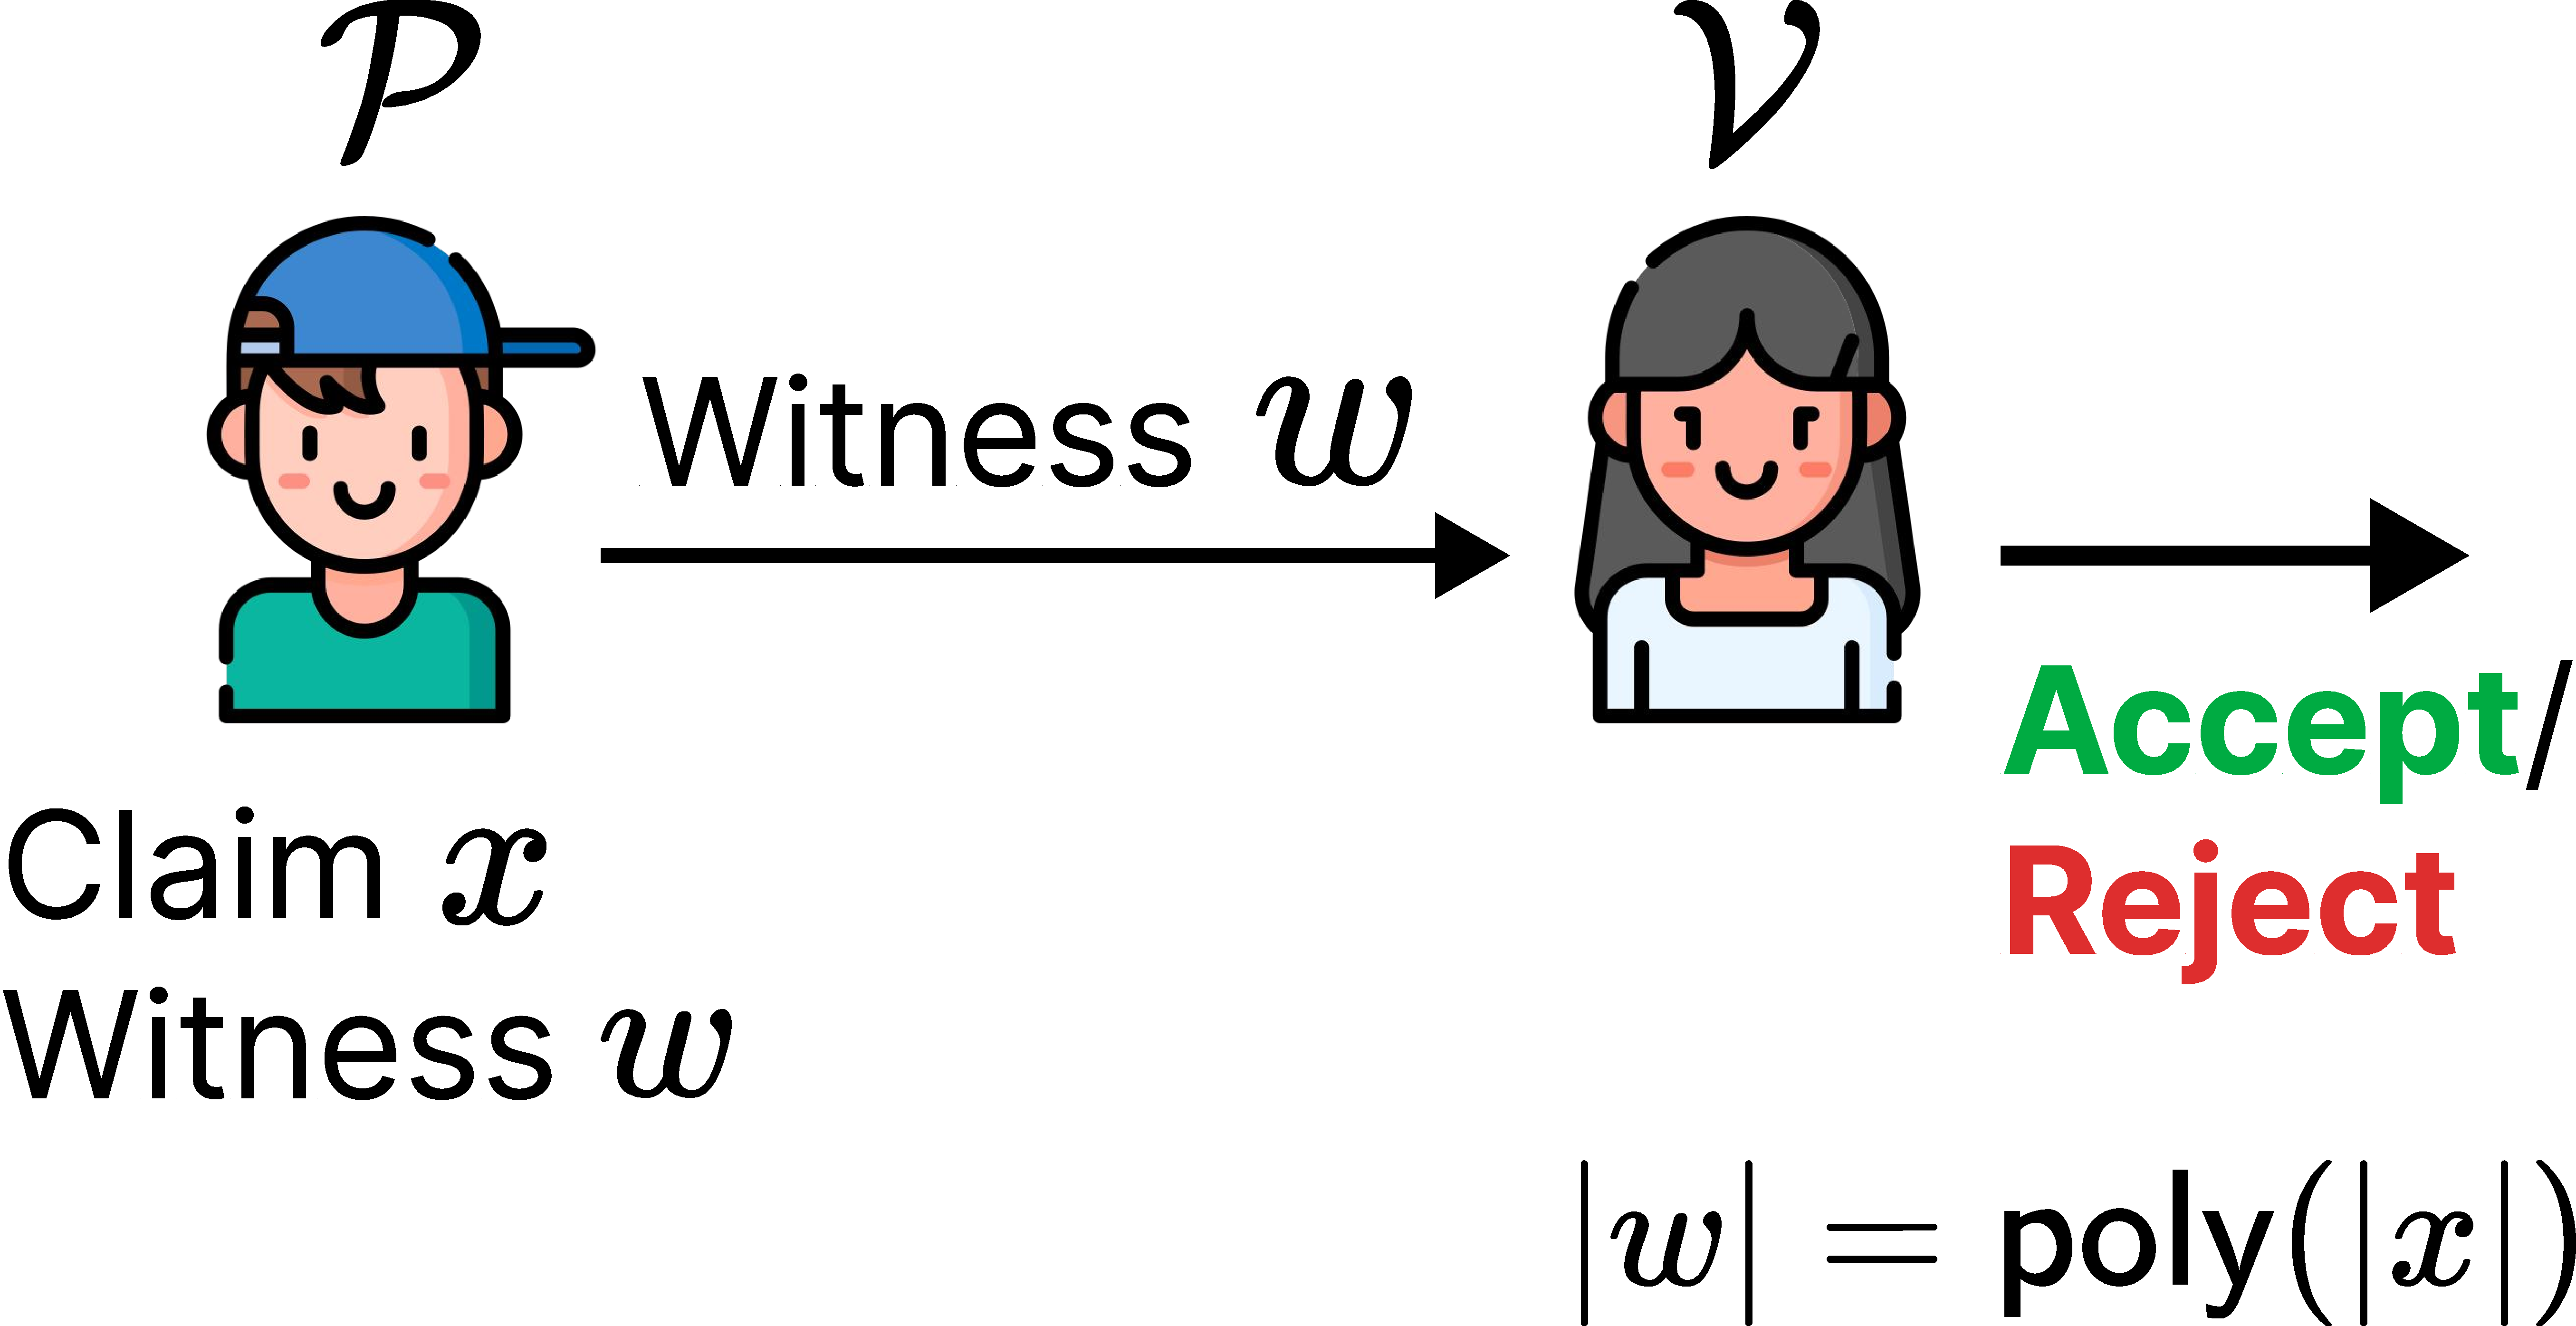
\includegraphics[width=0.7\textwidth]{images/lecture_6/np.pdf}
            \caption{Typical setup for cryptographic proofs.}
        \end{figure}
    \end{frame}

    \begin{frame}{NP Statements}
        \begin{definition}[P Language]
            Problem is in the $\mathbf{P}$ class if exists a polytime algorithm checking $x \in \mathcal{L}$.
        \end{definition}

        \begin{definition}[NP Language]
            A language $\mathcal{L}_{\mathcal{R}}$ belongs to the $\mathbf{NP}$ class if there exists a polynomial-time verifier $\mathcal{V}$ such that the following two properties hold:
            \begin{itemize}
                \item \textbf{Completeness:} If $x \in \mathcal{L}_{\mathcal{R}}$, then there is a witness $w$ such that $\mathcal{V}(x, w) = 1$ with $|w| = \mathsf{poly}(|x|)$. Essentially, it states that true claims have \textit{short} proofs.
                \item \textbf{Soundness:} If $x \not\in \mathcal{L}_{\mathcal{R}}$, then for any $w$ it holds that $\mathcal{V}(x, w) = 0$. Essentially, it states that false claims have no proofs.
            \end{itemize}
        \end{definition}

        \begin{theorem}
            Any $\mathbf{NP}$ problem has a zero-knowledge proof.
        \end{theorem}
    \end{frame}

    \begin{frame}{Question (aka Motivation)}
        But can we do better?

        Sending witness is\ldots Weird\ldots

        \begin{figure}
            \centering
            
\includegraphics[width=0.5\textwidth]{images/lecture_6/thonk.png}
            \caption{Hmm\ldots \#2}
        \end{figure}
    \end{frame}

    \section{Interactive Proofs}

    \subsection{Interactive Proof System}
    \begin{frame}{Solution!}
        \begin{columns}
            % Description
            \begin{column}{0.4\textwidth}
                We add two more ingredients:
                \begin{itemize}
                    \item \textbf{Interaction:} instead of \textbf{passively} receiving the proof, the verifier $\mathcal{V}$ can \textbf{interact} with the prover $\mathcal{P}$ by sending \textbf{challenges} and receiving \textbf{responses}.
                    \item \textbf{Randomness:} $\mathcal{V}$ can send random coins (challenges) to the prover, which $\mathcal{P}$ can use to generate responses.
                \end{itemize}
            \end{column}
            \begin{column}{0.6\textwidth}
                \begin{figure}
                    \centering
                    \begin{tikzpicture}[scale=0.90, transform shape]
                        \node[inner sep=0pt, align=center] (prover) {
\includegraphics[width=1.25cm]{images/lecture_6/prover.png}\\Prover $\mathcal{P}$\\\textbf{Comp. Unbounded}};
                        \node[inner sep=0pt, align=center, right=1.5cm of prover] (verifier) {
\includegraphics[width=1.25cm]{images/lecture_6/verifier.png}\\Verifier $\mathcal{V}$ \\ \textbf{Probabilistic} \\ \textbf{Poly-Time (PPT)}};
                
                        \draw [dashed,line width=0.3mm] ([yshift=-0.5cm]prover.south) -- ([yshift=-5.0cm]prover.south);
                        \draw [dashed,line width=0.3mm] ([yshift=-0.5cm]verifier.south) -- ([yshift=-4.8cm]verifier.south);
                
                        \draw[-{Stealth[length=3mm]},line width=0.4mm] ([yshift=-1.5cm]prover.south) coordinate (l2)--(l2-|verifier) node[midway, above=0mm, fill=white]{Send $m_1$};
                
                        \draw[-{Stealth[length=3mm]},line width=0.4mm] ([yshift=-2.25cm]verifier.south) coordinate (l2)--(l2-|prover) node[midway, above=1mm, fill=white]{Toss coin $r_1$, send query $q_1$};
                
                        \draw[-{Stealth[length=3mm]},line width=0.4mm] ([yshift=-3.5cm]prover.south) coordinate (l2)--(l2-|verifier) node[midway, above=0mm, fill=white]{Send $m_2$};
                
                        \draw[-{Stealth[length=3mm]},line width=0.4mm] ([yshift=-4.25cm]verifier.south) coordinate (l2)--(l2-|prover) node[midway, above=1mm, fill=white]{Toss coin $r_2$, send query $q_2$};
                    \end{tikzpicture}
                \end{figure}
            \end{column}
        \end{columns}
    \end{frame}

    \begin{frame}{Quadratic Residue Interactive Proof}
        \begin{block}{Problem Statement}
            \begin{itemize}
                \item \textbf{Statement:} $x \in \mathcal{L}_{\mathcal{R}}$ where our \textbf{language} is defined as:
                \begin{equation*}
                    \mathcal{L}_{\mathcal{R}} = \{x \in \mathbb{Z}_N^{\times}: \exists w \in \mathbb{Z}_N^{\times} \; \text{such that} \; x \equiv w^2 \; (\text{mod}\, N)\}
                \end{equation*}
                \item \textbf{Witness:} $w = \text{modular square root of $x$}$.
            \end{itemize}
        \end{block}

        How does $\mathcal{P}$ and $\mathcal{V}$ interact? Consider the figure below.

        \begin{figure}
            \centering
            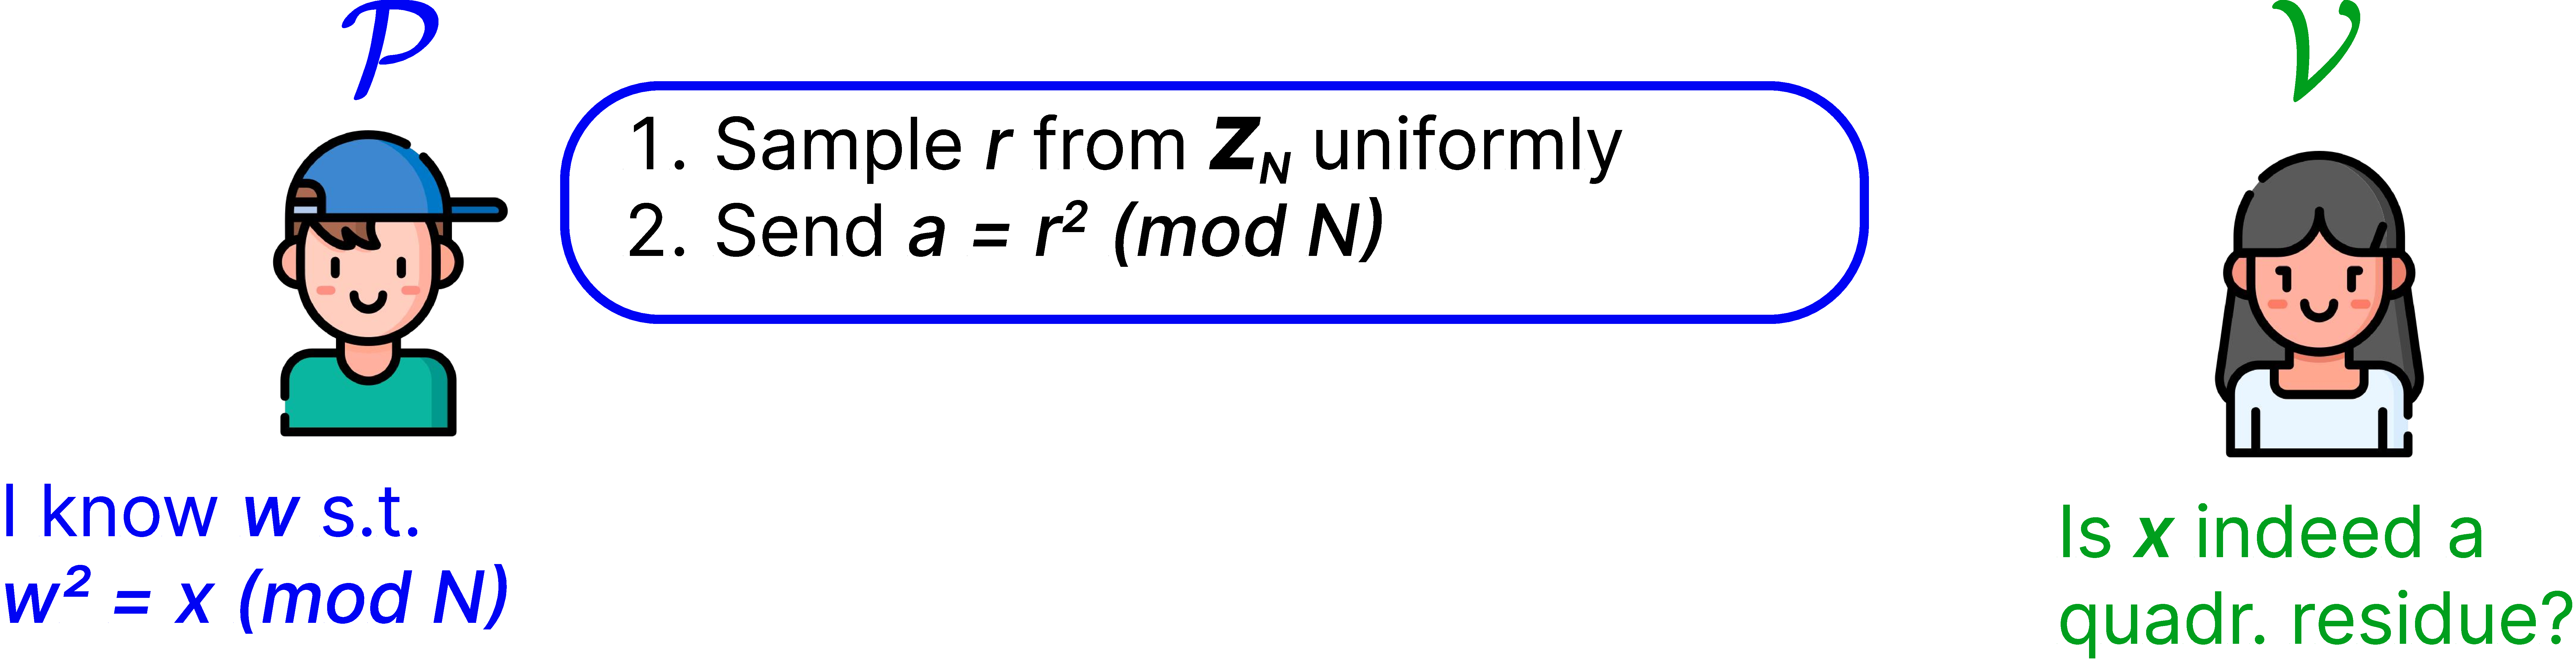
\includegraphics[width=\textwidth]{images/lecture_6/qr_test_1.pdf}
        \end{figure}
    \end{frame}

    \begin{frame}{Quadratic Residue Interactive Proof}
        \begin{figure}
            \centering
            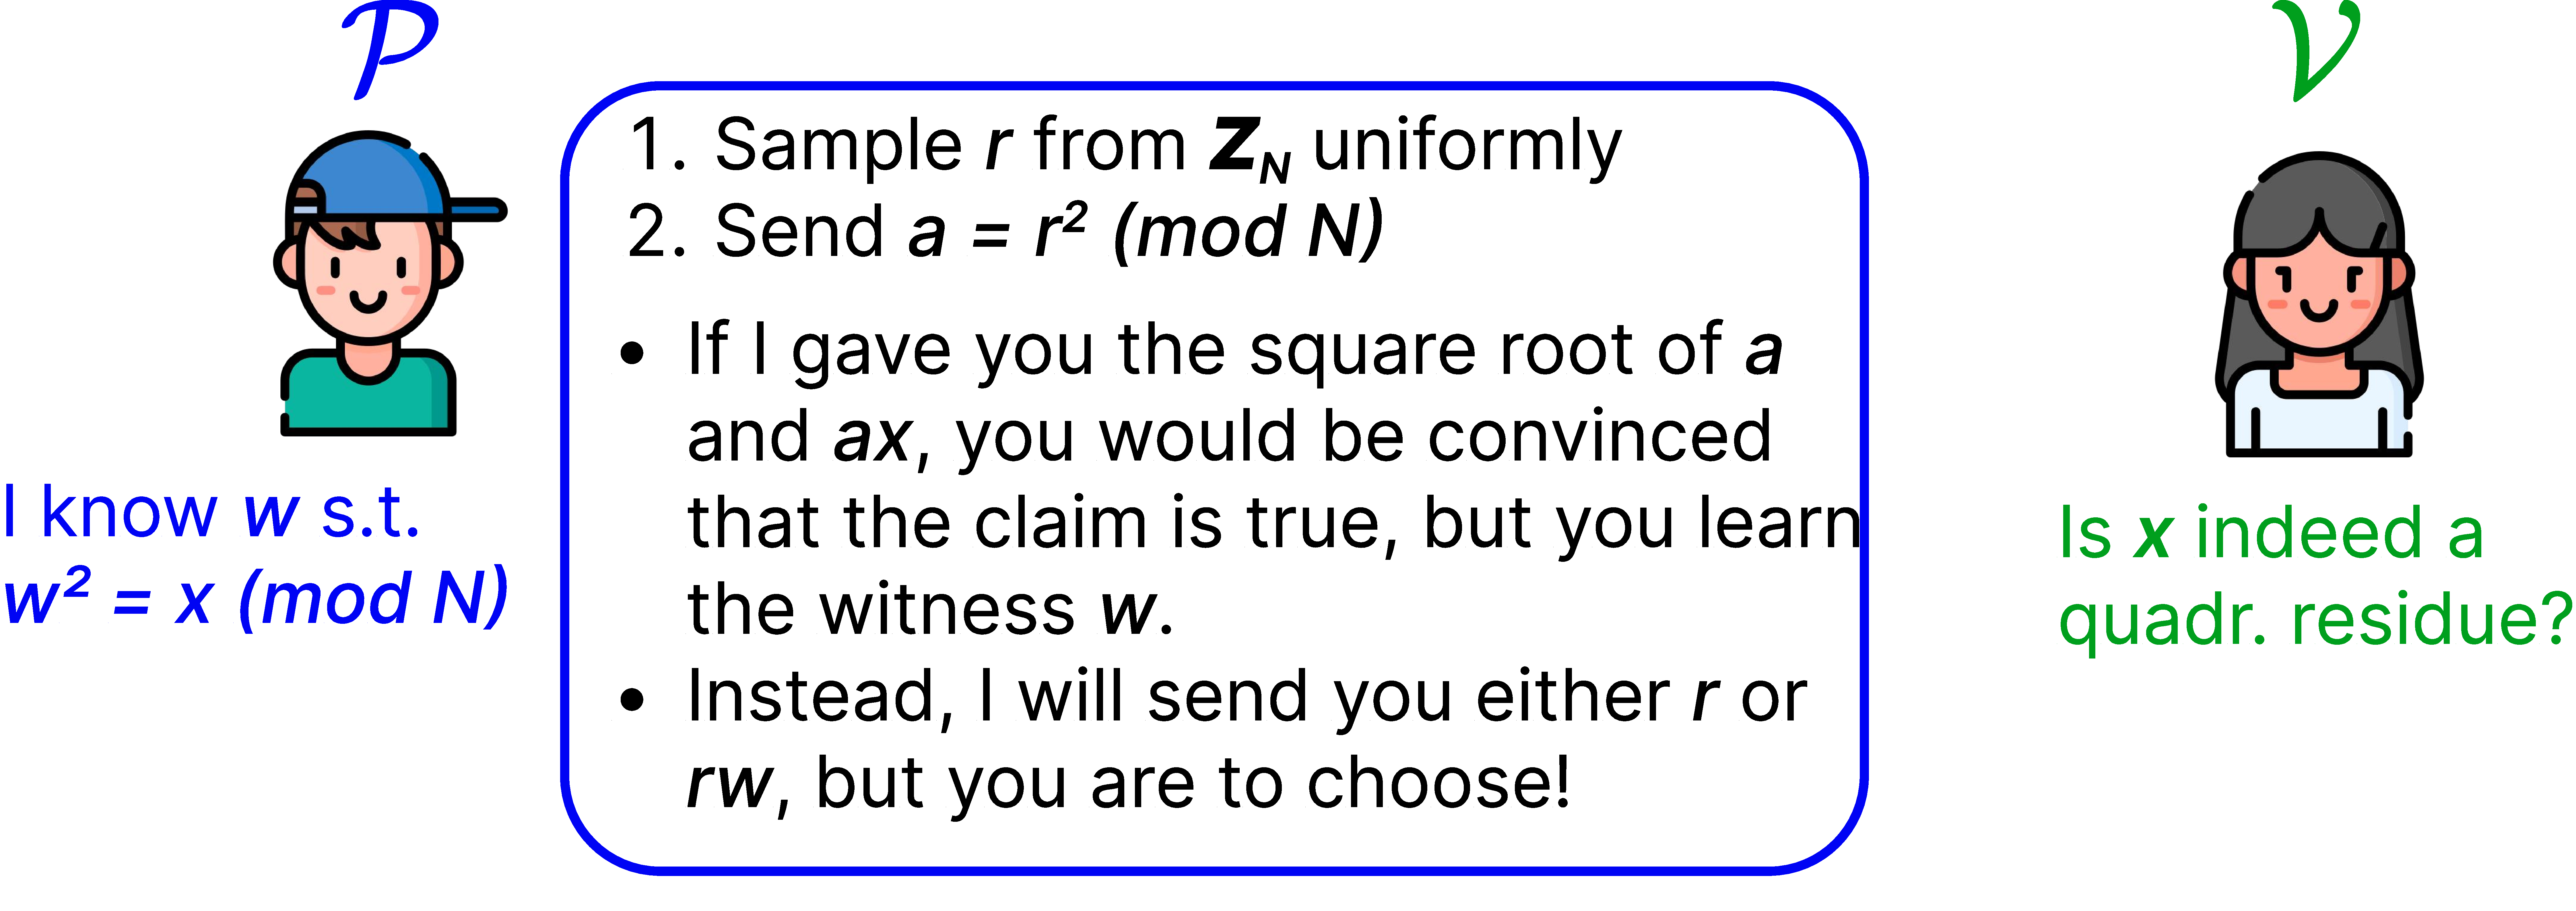
\includegraphics[width=\textwidth]{images/lecture_6/qr_test_2.pdf}
        \end{figure}
    \end{frame}

    \begin{frame}{Quadratic Residue Interactive Proof}
        \begin{figure}
            \centering
            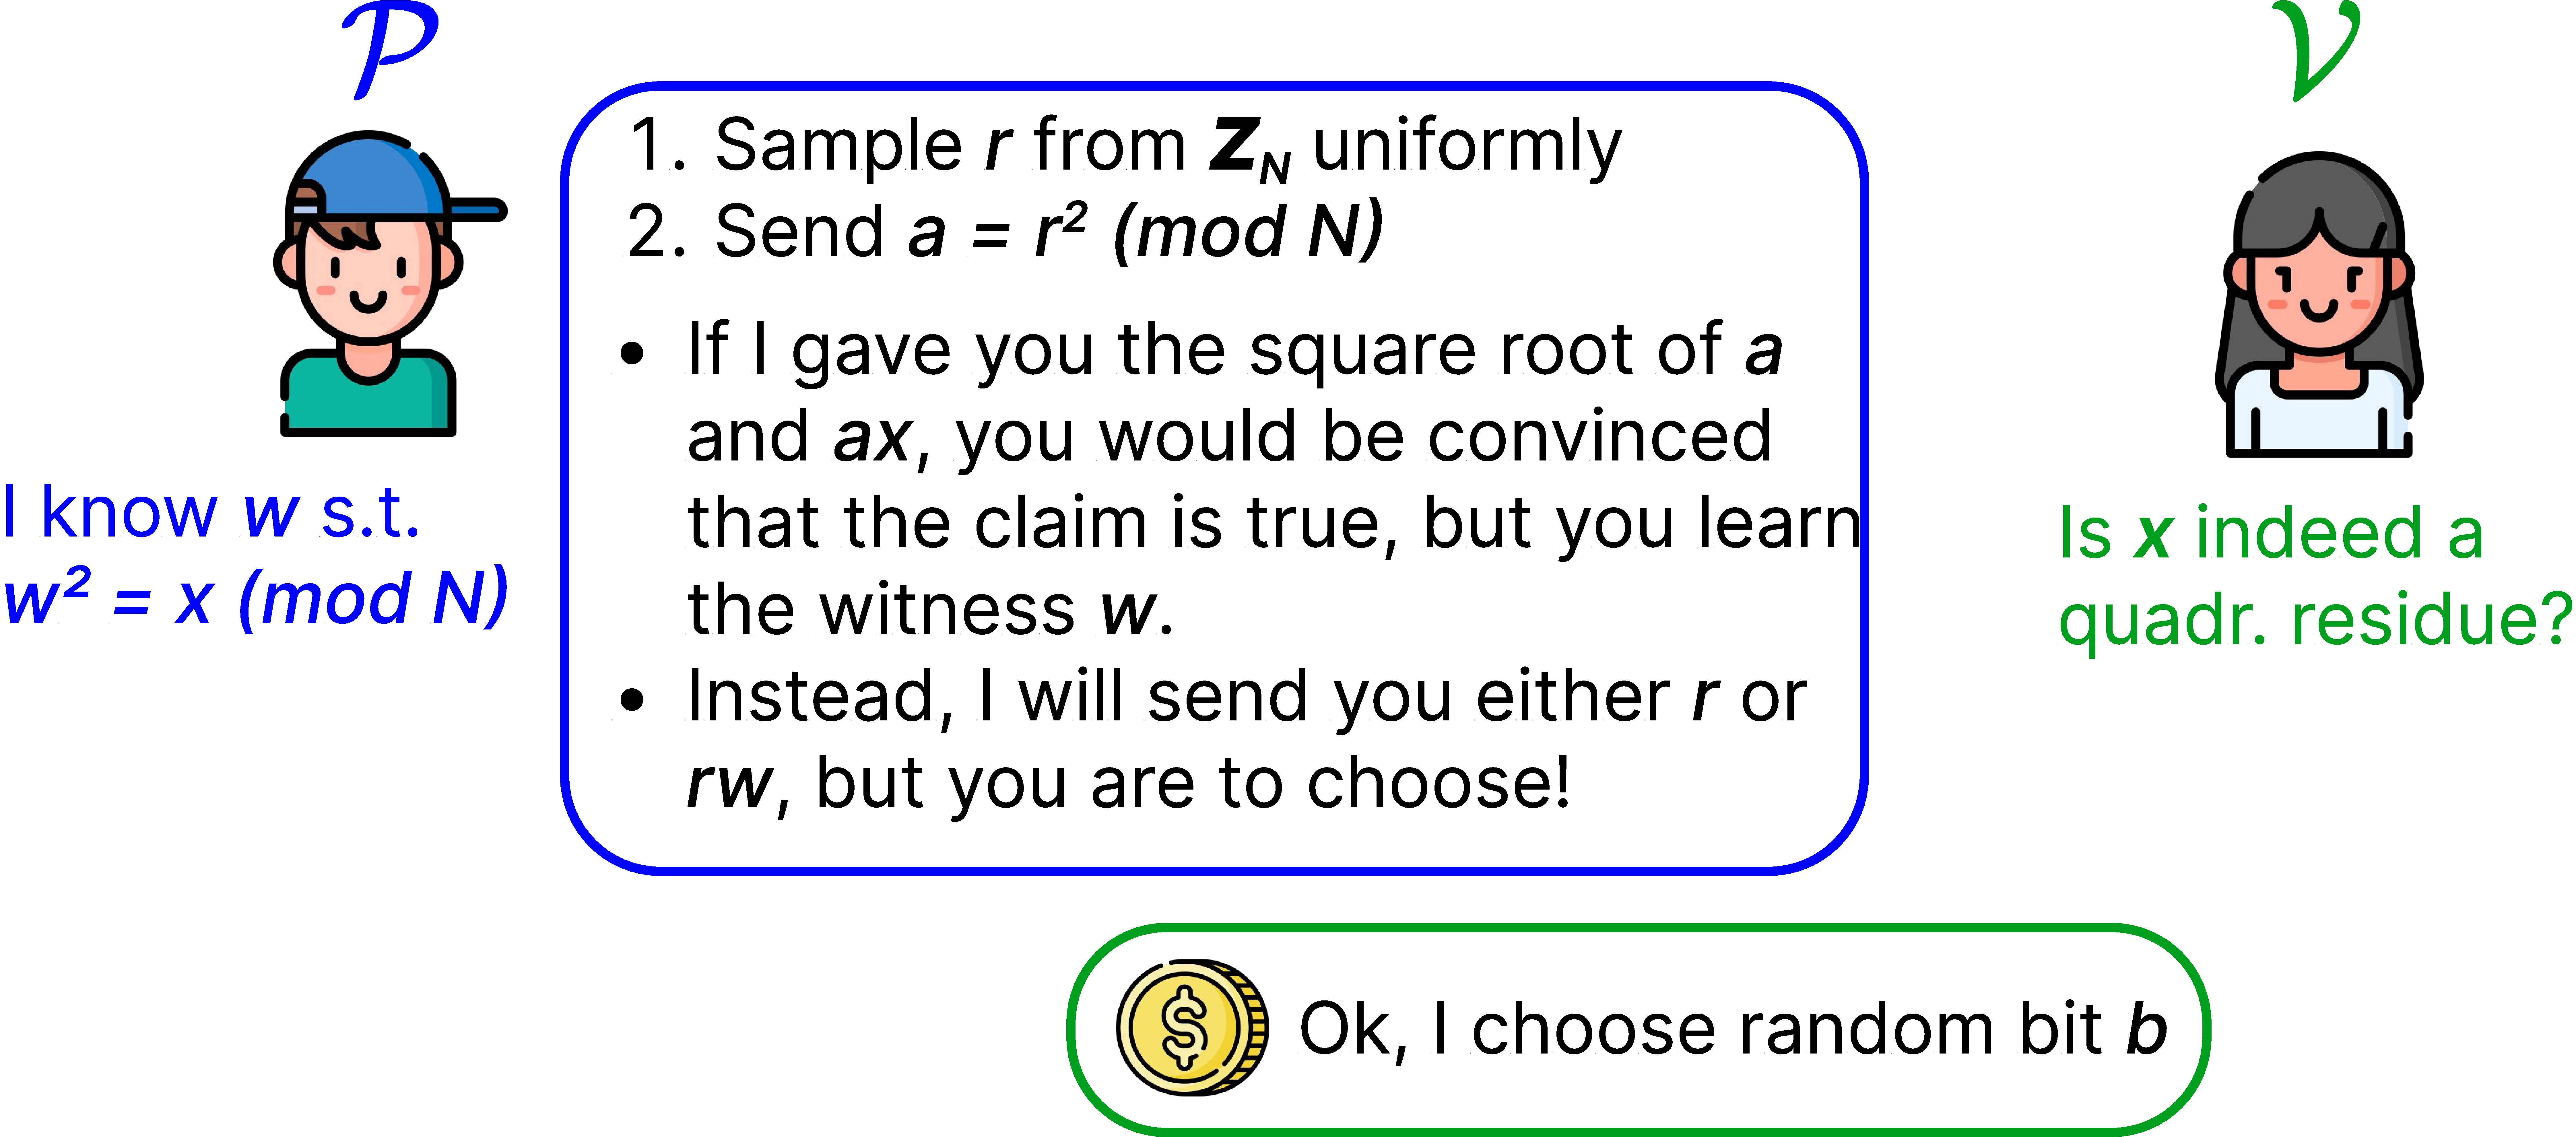
\includegraphics[width=\textwidth]{images/lecture_6/qr_test_3.pdf}
        \end{figure}
    \end{frame}

    \begin{frame}{Quadratic Residue Interactive Proof}
        \begin{figure}
            \centering
            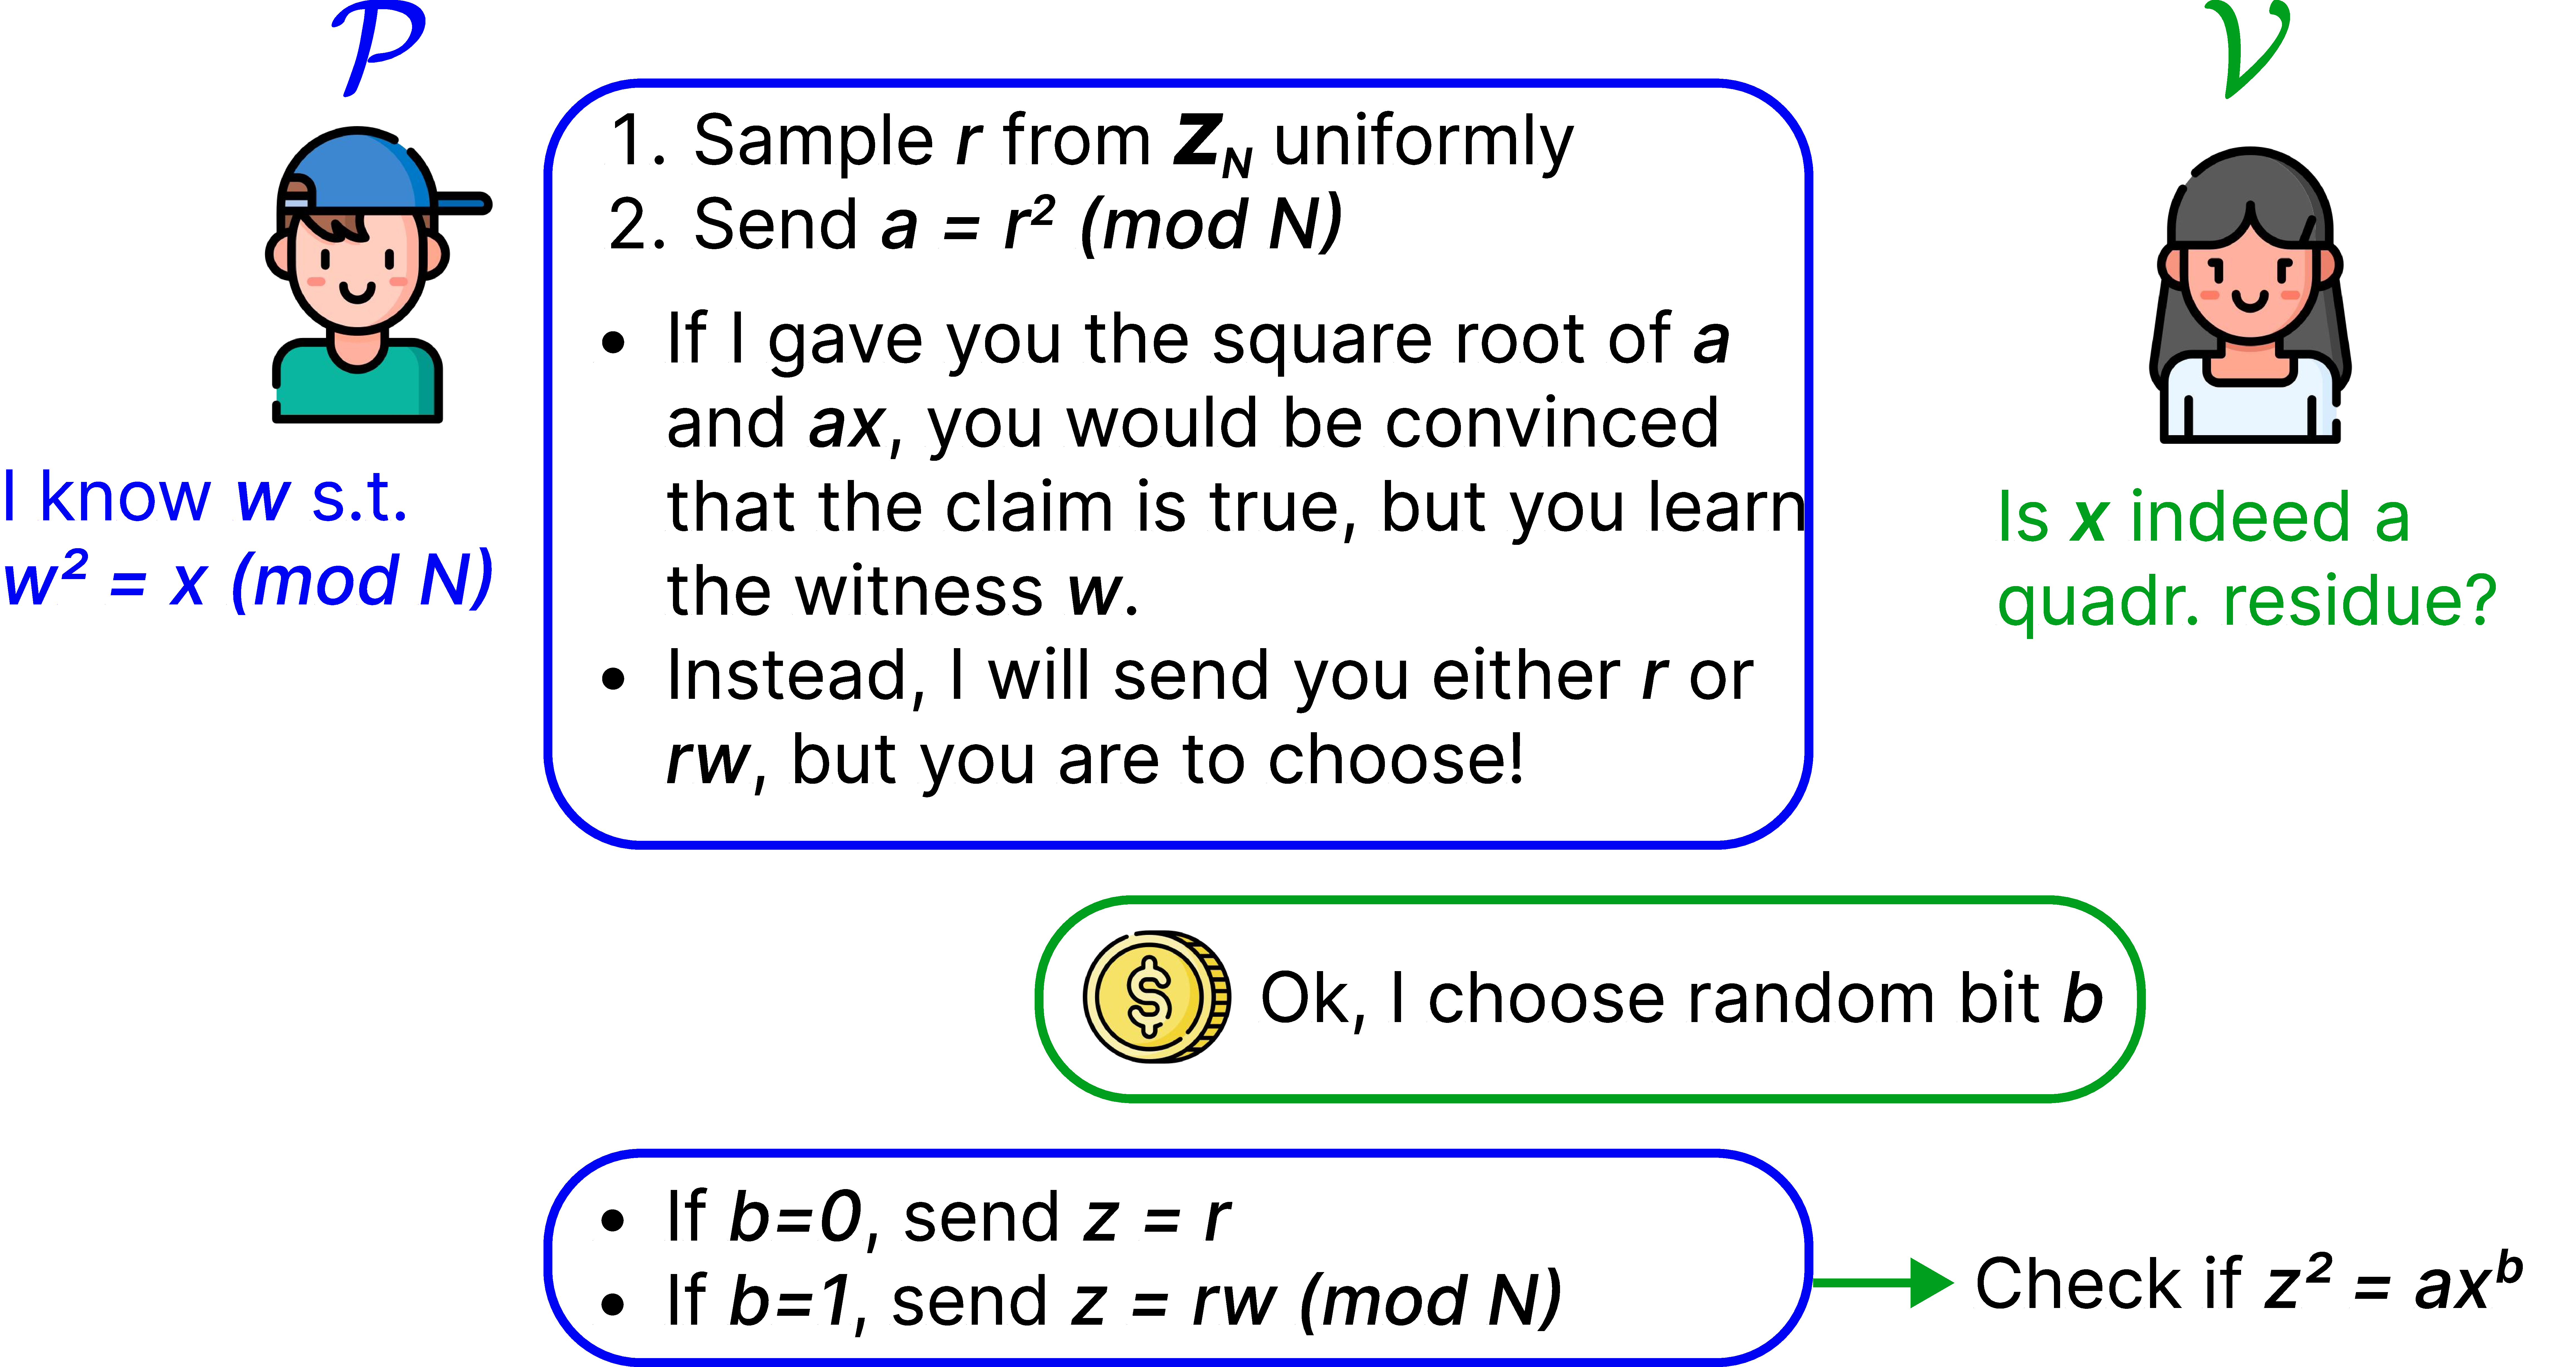
\includegraphics[width=\textwidth]{images/lecture_6/qr_test_4.pdf}
        \end{figure}
    \end{frame}

    \begin{frame}{Quadratic Residue Interactive Proof: Analysis}
        \begin{block}{Interactive Protocol}
            \begin{enumerate}
                \item $\mathcal{P}$ samples $r \xleftarrow{R} \mathbb{Z}_N^{\times}$ and sends $a = r^2$ to $\mathcal{V}$.
                \item $\mathcal{V}$ sends a random bit $b \in \{0,1\}$ to $\mathcal{P}$.
                \item $\mathcal{P}$ sends $z = r \cdot w^b$ to $\mathcal{V}$.
                \item $\mathcal{V}$ accepts if $z^2 = a \cdot x^b$, otherwise it rejects.
                \item Repeat $\lambda \in \mathbb{N}$ times.
            \end{enumerate}
        \end{block}

        \begin{lemma}
            The protocol is \textbf{complete} and \textbf{sound}.
        \end{lemma}

        \textbf{Completeness.} If $b=0$, then $z=r$ and thus $z^2=r^2=a$, check passes.

        If $b=1$, then $z=rw$ and thus $z^2=r^2w^2=ax$, check passes.
    \end{frame}

    \begin{frame}{Quadratic Residue Interactive Proof: Analysis}
        \textbf{Soundness.} The main reason why the protocol is sound is insribed in the theorem below.

        \begin{theorem}
            For any prover $\mathcal{P}^*$ with $x \not\in \mathcal{L}_{\mathcal{R}}$, the probability of $\mathcal{V}$ accepting the proof is at most $1/2$. 
        \end{theorem}

        \textbf{Corollary.} After repeating the protocol $\lambda$ times, we have
        \begin{equation*}
            \text{Pr}[\mathcal{V} \; \text{accepts after $\lambda$ rounds}] \leq \frac{1}{2^{\lambda}} = \mathsf{negl}(\lambda).
        \end{equation*}

        Thus, we showed both \textbf{completeness} and \textbf{soundness} of the protocol.
    \end{frame}

    \begin{frame}{Interactive Protocol Definition}
        \textcolor{gray}{$\langle \mathcal{P}, \mathcal{V} \rangle(x)$ reads as ``interaction between $\mathcal{P}$ and $\mathcal{V}$ on the statement $x$''.}

        \begin{definition}
            A pair of algorithms $(\mathcal{P},\mathcal{V})$ is called an \textbf{interactive proof} for a language $\mathcal{L}_{\mathcal{R}}$ if $\mathcal{V}$ is a polynomial-time verifier and the following two properties hold:
            \begin{itemize}
                \item \textbf{Completeness:} For any $x \in \mathcal{L}_{\mathcal{R}}$, $\text{Pr}[\langle \mathcal{P}, \mathcal{V} \rangle(x) = \mathsf{accept}]=1$.
                \item \textbf{Soundness:} For any $x \not\in \mathcal{L}_{\mathcal{R}}$ and for any prover $\mathcal{P}^*$, we have 
                \begin{equation*}
                    \text{Pr}[\langle \mathcal{P}^*, \mathcal{V} \rangle(x) = \mathsf{accept}] \leq \mathsf{negl}(\lambda)
                \end{equation*}
            \end{itemize}
        \end{definition}

        \begin{definition}
            \textbf{The class of interactive proofs} (\textbf{IP}) is defined as:
            \begin{equation*}
                \mathbf{IP} = \{\mathcal{L}: \text{there is an interactive proof $(\mathcal{P}, \mathcal{V})$ for $\mathcal{L}$}\}.
            \end{equation*}
        \end{definition}
    \end{frame}

    \begin{frame}{Zero-Knowledge Informal Definition}
        \begin{definition}
            An interactive proof system $(\mathcal{P}, \mathcal{V})$ is called \textbf{zero-knowledge} if for any polynomial-time verifier $\mathcal{V}^*$ and any $x \in \mathcal{L}_{\mathcal{R}}$, the interaction $\langle \mathcal{P}, \mathcal{V}^* \rangle(x)$ gives nothing new about the witness $w$.
        \end{definition}
        
        \begin{definition}
            The pair of algorithms $(\mathcal{P}, \mathcal{V})$ is called a \textbf{zero-knowledge interactive protocol} if it is \textit{complete}, \textit{sound}, and \textit{zero-knowledge}.
        \end{definition}

        \begin{figure}
            \centering
            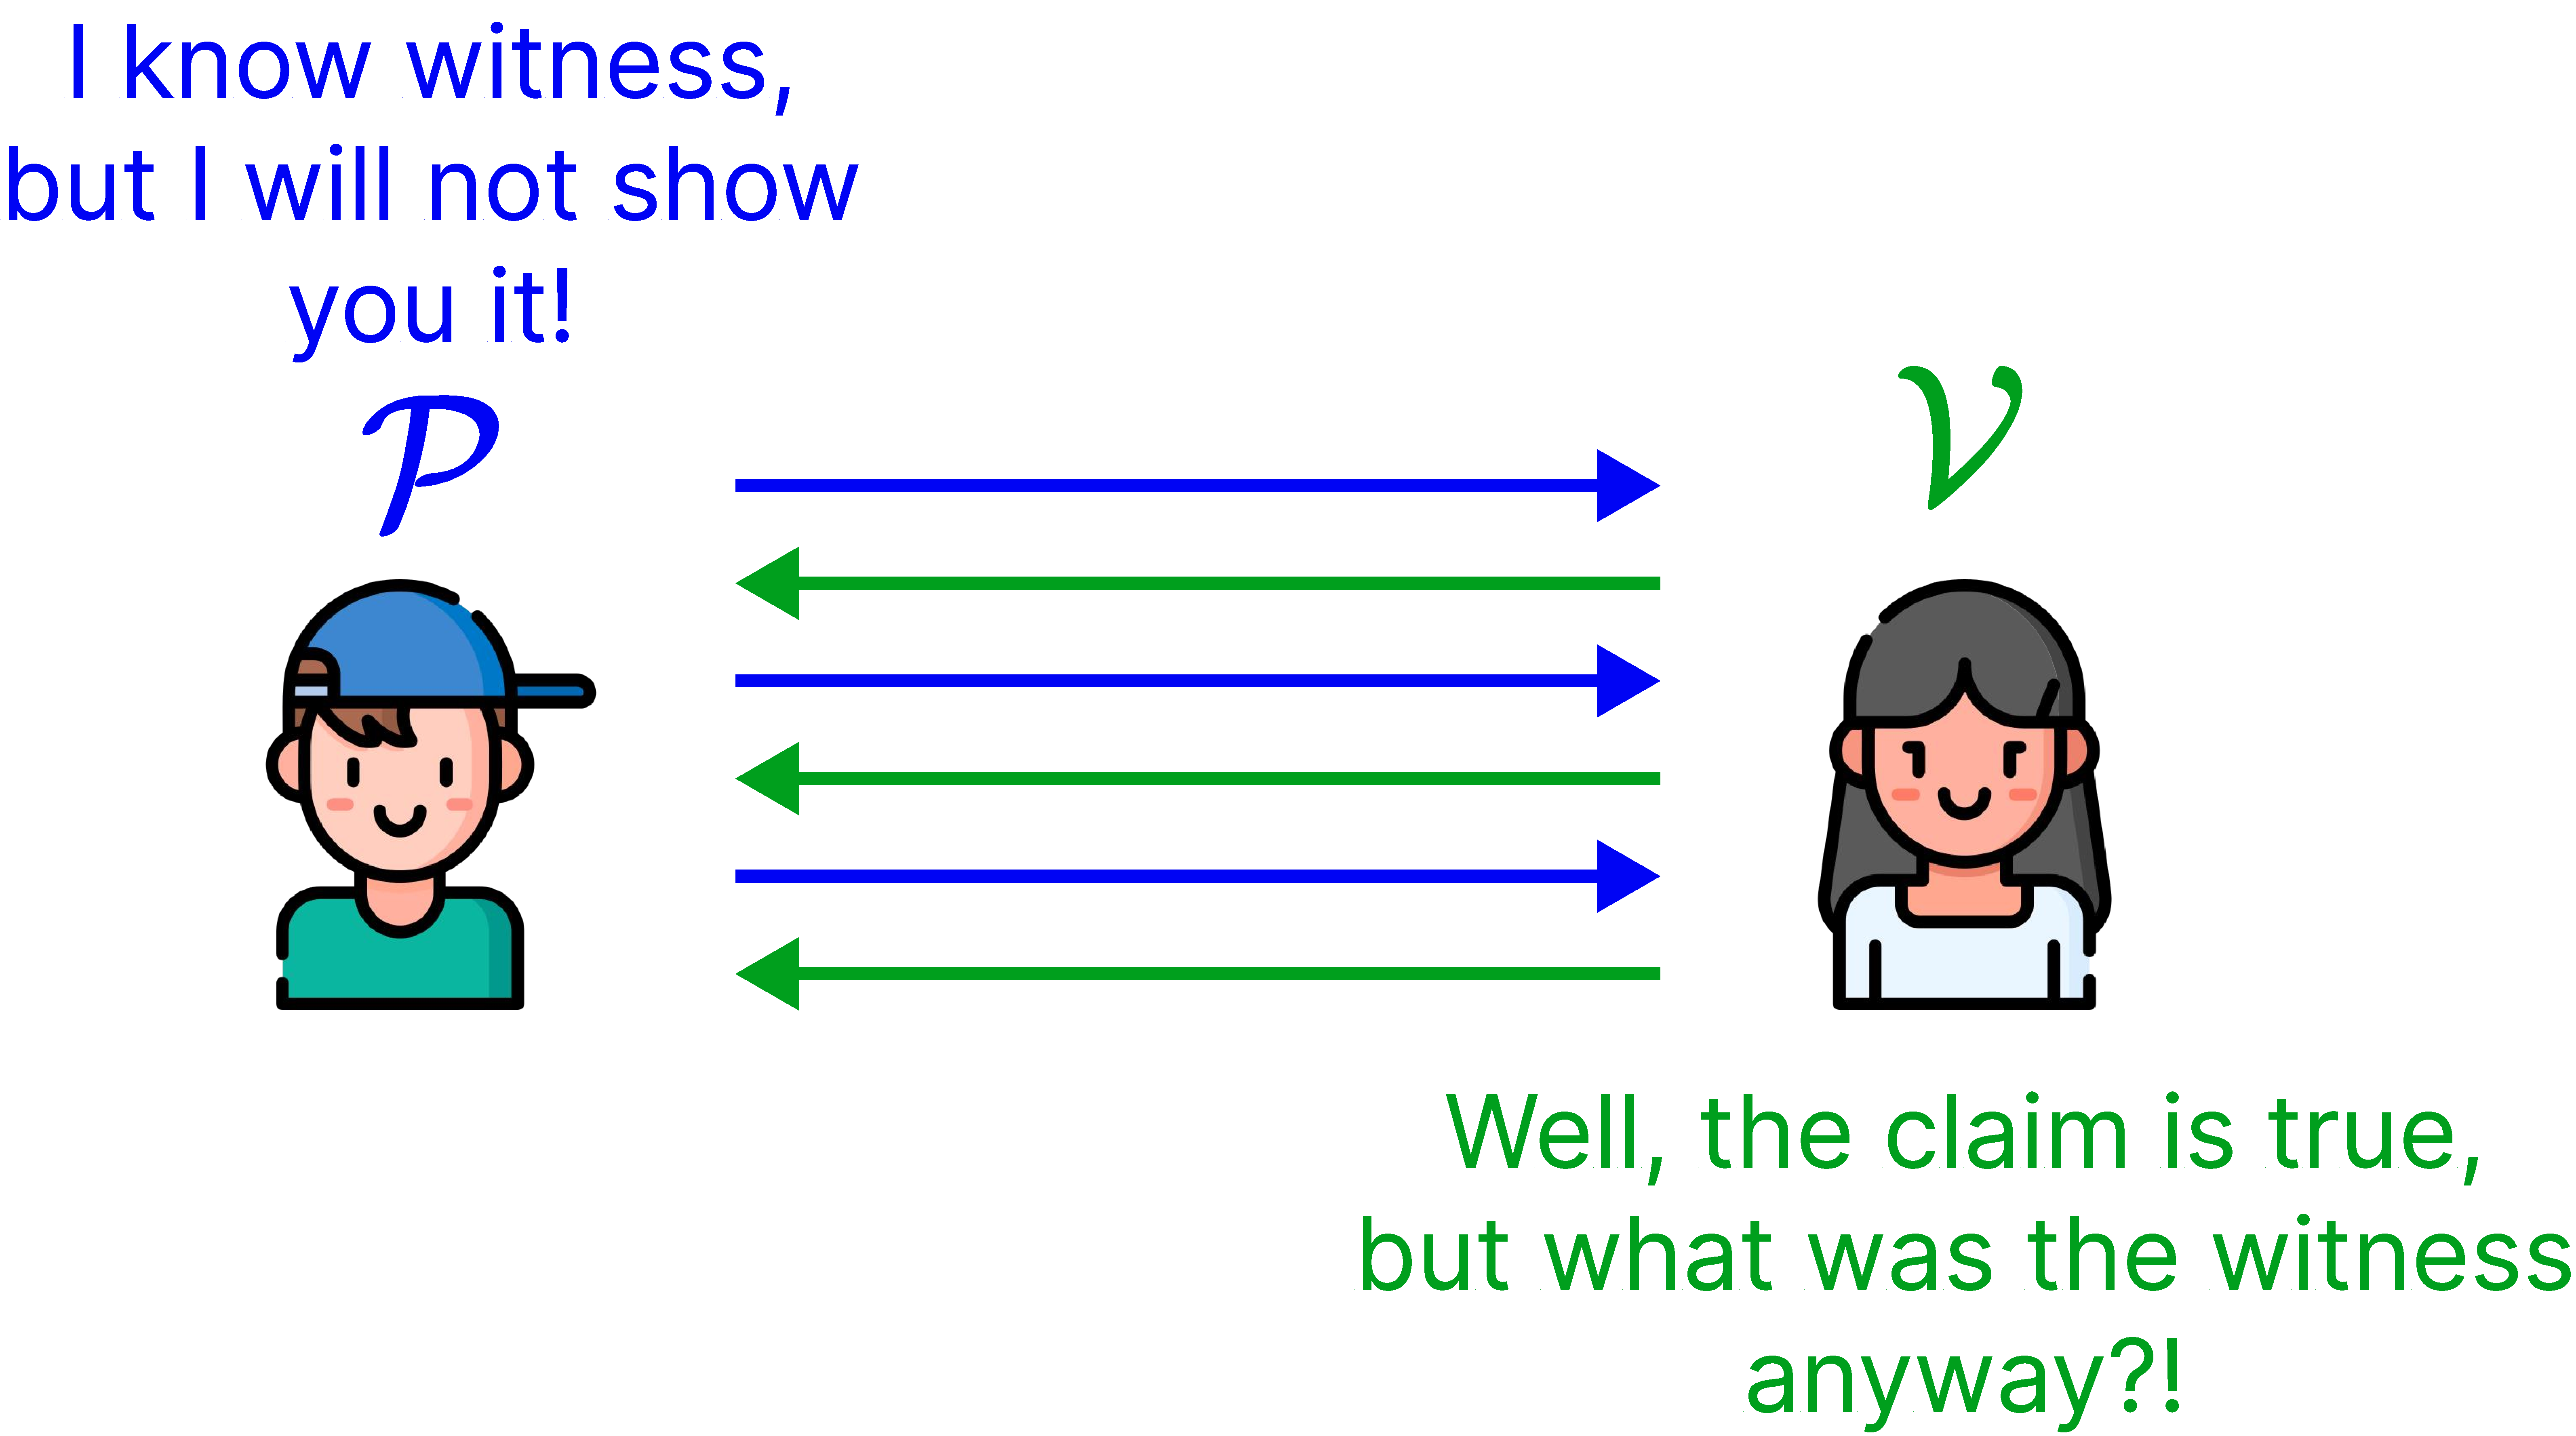
\includegraphics[width=0.5\textwidth]{images/lecture_6/zk.pdf}
        \end{figure}
    \end{frame}

	\begin{frame}{}
      \centering \Large
      \emph{Thanks for your attention!}
    \end{frame}
\end{document}